\chapter{Введение}

Современные технологии систем умных домов предоставляют уникальные возможности для автоматизации и управления различными аспектами жилища, обеспечивая комфорт, безопасность и энергоэффективность. В данной работе был проведен анализ целевой аудитории проекта, с целью определения потребностей и предпочтений пользователей. 

Наша задача была разработать систему «Умный дом».  Система в виде стенда с датчиками, которые отображают её работу. Также, в эту систему входят камеры, которые отправляют информацию о безопасности в наш Телеграмм бот. 

В рамках исследования,  было изучено применение системы компьютерного зрения в проекте, включая роль и необходимость искусственного интеллекта, различные типы искусственного  интеллекта, выбор языка программирования и библиотеки, а также этапы реализации данной технологии.

Далее разработка web-сайта с анализом существующих страниц, созданием дизайна интерфейса, frontend и backend разработкой. Создание бота в Telegram, включая использованные материалы, функционал и цели данного проекта. Соединением сайта с датчиками также было реализовано.

Каждый раздел представляет собой важный этап в разработке и реализации системы умного дома, направленный на обеспечение удобства, эффективности и современных технологических решений для пользователей.

\chapter{Анализ целевой аудитории проекта.}

Для определения нашей целевой аудитории мы провели анализ рынка.

\begin{figure}[h!]
	\centering
	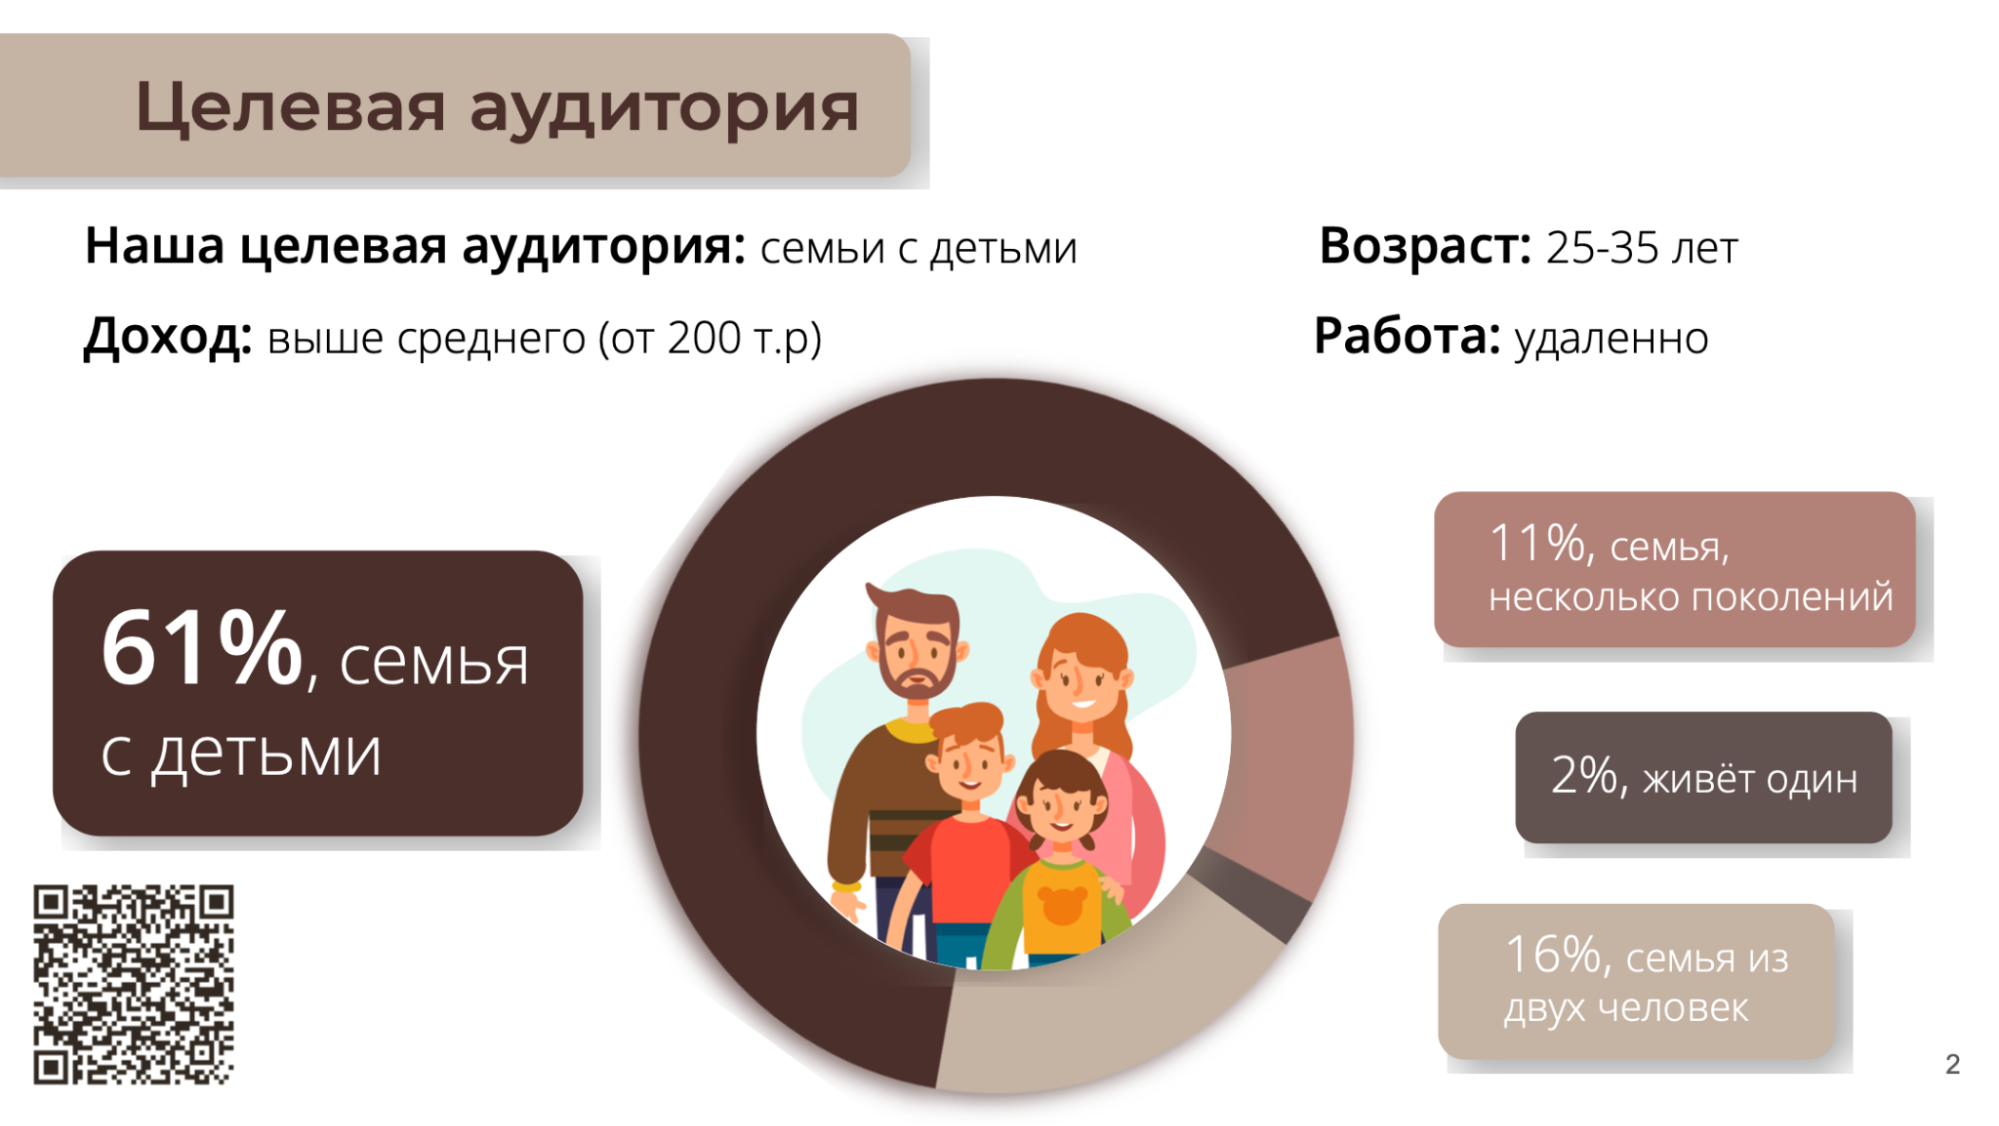
\includegraphics[width=0.8\textwidth]{./graphics/img/image32.png}
	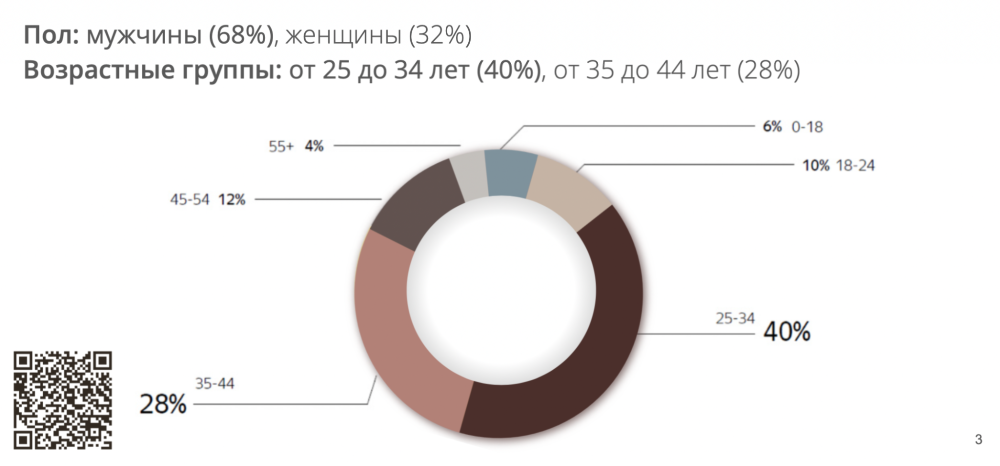
\includegraphics[width=0.8\textwidth]{./graphics/img/image14.png}
	\caption{статистические данные для анализа целевой аудитории.}
\end{figure}

Основываясь на статистических данных можно сделать вывод о том, что наибольшей группой покупателей системы умного дома являются мужчины в возрасте от 25 до 34 лет [1]. Также благодаря статистическим данным мы выявили, что 61\% покупателей умных домов являются семьи с детьми[2]. Помимо этого, мы прописали, что жители наших умных коттеджей должны работать удалённо. Это связано с тем, что коттеджные поселки находятся вдали от центра города. Люди, работающие в офисах предпочитают выбирать жилье, которое находится как можно ближе к их работе, следовательно им будет гораздо комфортнее жить в жилых комплексах в квартире. Но, если у покупателей коттеджей нет привязки к месту (работаю удалённо), им нет смысла стремиться купить дом ближе к центру. 

Помимо этого, при анализе рынка мы выявили основные запросы нашей целевой аудитории:

\begin{enumerate}
	\item Безопасность. Благодаря системе видеонаблюдения с распознаванием силуэта человека, а также датчику утечки газа, семья может быть спокойна за безопасность своих близких. 
	\item Климат-контроль. Благодаря датчикам температуры и влажности пользователь сможет отслеживать данные с них на сайте.  
	\item Удобство и комфорт. Коттеджный поселок располагается в удобном для проживания месте. Также есть несколько планов домов, которые смогут удовлетворить потребности разных семей. 
	\item Дистанционное управление. Владельцы смогут управлять умным домом через Telegram-bot,  а также отслеживать данные с датчиков через сайт.  
	\item Помощь по дому. Умный робот будет помогать убирать игрушки за детьми.
\end{enumerate}

\chapter{Создание системы “Умный дом”}

\section{Внешний вид стенда Умный дом}

\begin{figure}[h!]
    \centering
	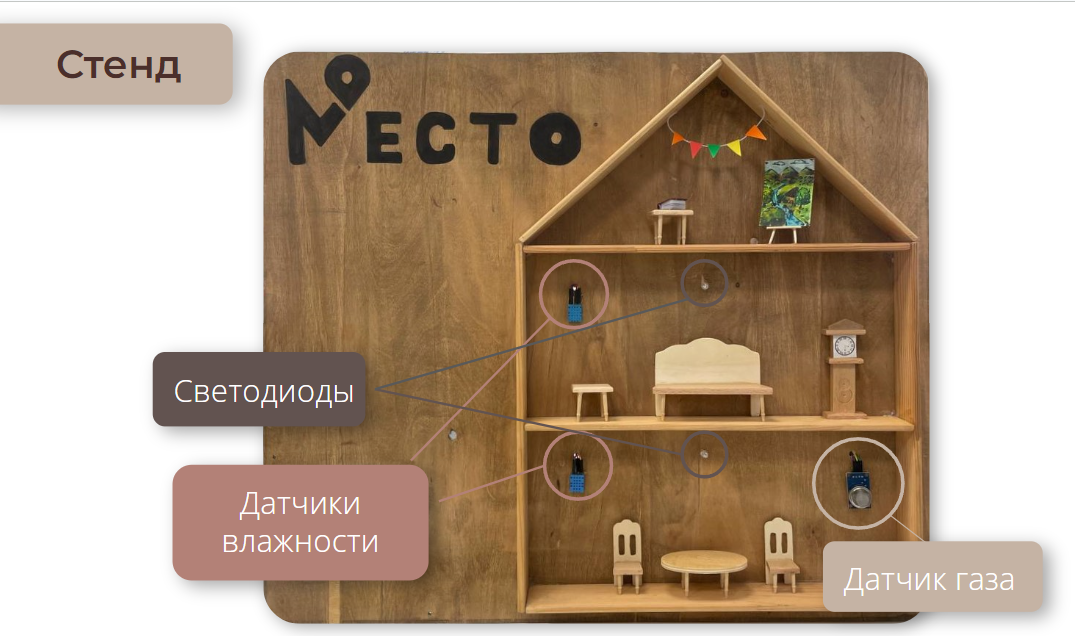
\includegraphics[width=0.8\textwidth]{./graphics/img/image13.png}
	\caption{Внешний вид нашего стенда}
	\label{fig:img13}
\end{figure}

Стенд нашего умного дома сделан из фанерного листа покрытого морилкой. Фигура дома сделана из нарезанных деревянных дощечек скрепленных между собой двухкомпонентным клеем. В условном доме стенде размещена декоративная мебель, которая указывает на расположение гостевой зоны на первом этаже и зоны отдыха на втором этаже. На каждом этаже расположены датчики влажности и светодиоды. На первом этаже в зоне кухни расположен датчик утечки газа. Провода и микроконтроллер ESP32 закреплены на задней стенке стенда.
\clearpage

\section{Алгоритм работы системы «Умный дом»}

\begin{figure}[h!]
	\centering
	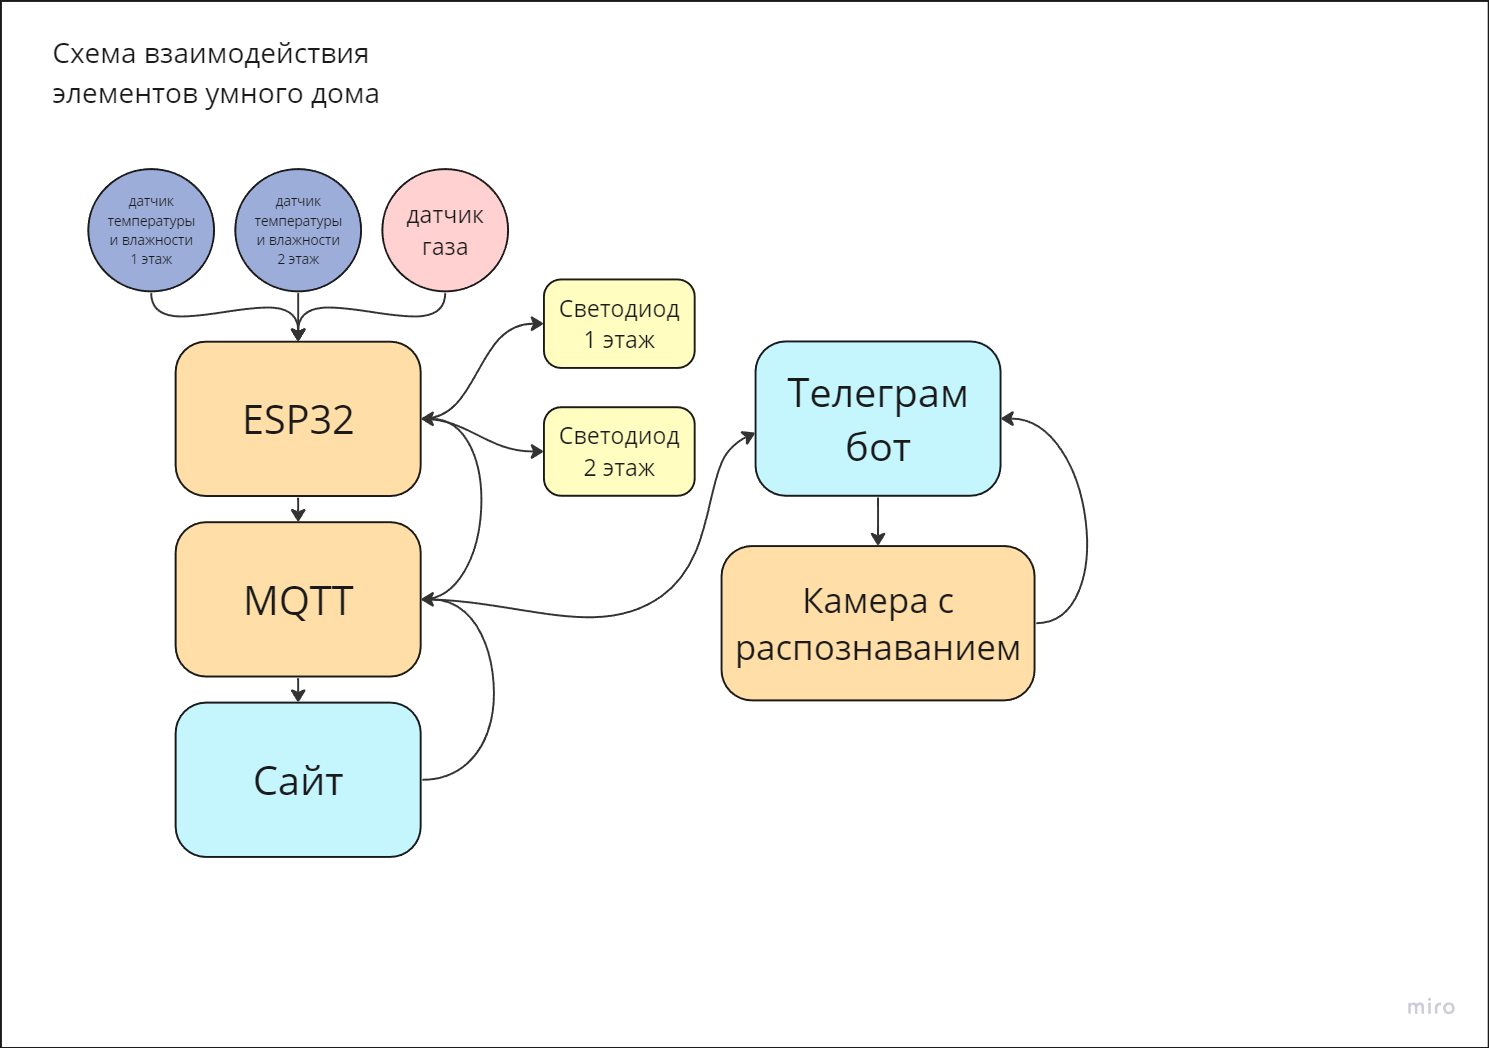
\includegraphics[width=0.8\textwidth]{./graphics/img/image25.png}
	\caption{алгоритм работы системы «Умный дом».}
	\label{fig:img25}
\end{figure}

На рисунке \ref{fig:img25} мы видим, что микроконтроллер получает данные с двух датчиков температуры и влажности DHT11 и управляет двумя трехцветными светодиодами. При этом ESP32 обменивается данными с mqtt сервером. С mqtt сервера данные поступают с датчиков поступают на сайт и телеграм бота. С сайта производится включение и выключения светодиодов, имитируя свет в доме. На телеграм бота поступают данные с датчиков температуры и влажности и газа, обратно бот не отдает никакие данные. С телеграм бота пользователь может узнать данные с датчиков и взаимодействовать с камерой которая распознает силуэты людей.

\section{Датчики и серверная часть системы}

\subsection{Используемые программы}

\begin{description}
	\item[Mosquitto] — локальный mqtt брокер, позволяющий сайту, телеграм-боту и стенду на esp32 обмениваться данными.
	\item[Thonny IDE] — интегрированная среда разработки для языка micropython, необходимая для написания и отладки кода микроконтроллера, а также последующей прошивки устройства.
	\item[nano] — консольный текстовый редактор, необходимый для исправления конфигурационных файлов и подготовки системы для установки прочих программ.
	\item[emerge] — интерфейс командной строки для portage, пакетного менеджера ОС gentoo по-умолчанию, необходимый для установки программ и библиотек, а также для управления их зависимостями.
	\item[nmcli] —  интерфейс командной строки для Network Manager, программы для управления сетевыми подключениями в ОС, основанных на GNU/Linux, необходимый для переключения в зависимости от ситуации между глобальной сетью Интернет и локальной сетью, которую создавала esp32.
	\item[ip] — консольная утилита, позволяющая узнать свой локальный IP, необходимый для подключения микроконтроллера к mqtt брокеру.
	\item[lsof] — консольная утилита, позволяющая узнать процессы в системе, занимающие определенные сетевые порты. Данная информация была необходима для исследования системы и управления различными версиями сайта, запущенными параллельно для сравнительного анализа и разработки наилучшей комбинации различных решений.
	\item[rm] — консольная утилита, необходимая для удаления ошибочно созданных и мешающих файлов.
	\item[mkdir] —  консольная утилита, необходимая для создания новых директорий для проекта.
	\item[micropython] — консольный интерфейс для REPL, среды исполнения языка micropython.
	\item[esptool] —  консольная утилита для прошивки микроконтроллеров esp.
\end{description}

\subsection{Логика работы}
\mbox{}
\begin{figure}[h!]
	\centering
	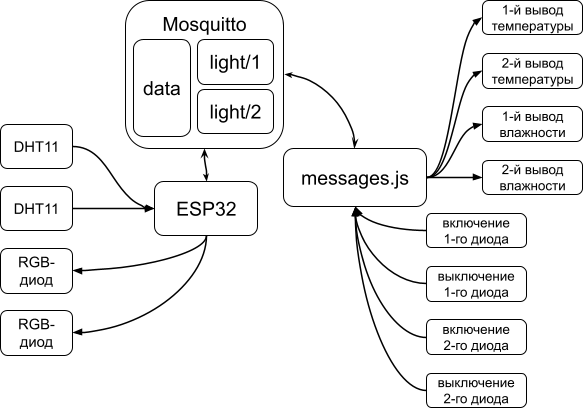
\includegraphics[width=0.8\textwidth]{./graphics/img/image36.png}
	\caption{Схема логики работы}
	\label{fig:img36}
\end{figure}

На схеме видно, что микроконтроллер получает данные с двух датчиков температуры и влажности DHT11 и управляет двумя трехцветными светодиодами. При этом ESP32 обменивается данными с mqtt сервером Mosquitto, отправляя данные с датчиков в топик data и читая из топиков light/1 и light/2.

Сайт представлен здесь файлом messages.js и несколькими элементами верстки, связанными с ним. Подробнее его устройство будет рассмотрено в разделе Backend сайта.

Рассмотрим подробнее логику работы ESP32. Как было указано выше, для программирования микроконтроллера использовались IDE thonny и язык программирования micropython (далее ЯП или micropy). В micropy большая часть функционала вынесена в библиотеки, поэтому их пришлось активно использовать при программировании. Так для взаимодействия и управления светодиодами использовалась функция Pin библиотеки machine, для взаимодействия с датчиками использовалась библиотека dht. Также использовались библиотеки network для сети, umqtt.simple для передачи данных и time для выставления задержки между снятиями показателей или запросом новых статусов для светодиодов. На рисунке 6 представлены импорты необходимых компонентов.

\begin{figure}[h!]
	\centering
	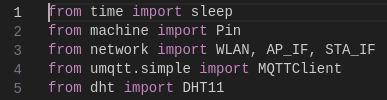
\includegraphics[width=0.5\textwidth]{./graphics/img/image37.png}
	\caption{Импорты необходимых компонентов}
	\label{fig:img37}
\end{figure}

\begin{figure}[h!]
	\centering
	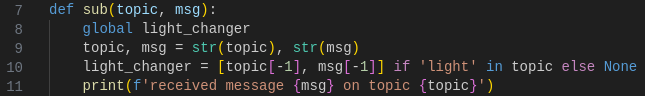
\includegraphics[width=0.8\textwidth]{./graphics/img/image31.png}
	\caption{функция для обработки входящих сообщений}
	\label{fig:img31}
\end{figure} 

На рисунке \ref{fig:img37} показана функция для обработки входящих сообщений. Здесь используется редактирование глобальной переменной light\_changer из-за особенностей реализации umqtt.simple. В неё помещаются последние символы из переменных topic \& msg, которые должны являться целыми числами, которые обозначают номер светодиода (1 или 2) и его состояние (0 – выключен и 1 – включён). Также выводится отладочное сообщение об успешности получения сообщения.

\begin{figure}[h!]
	\centering
	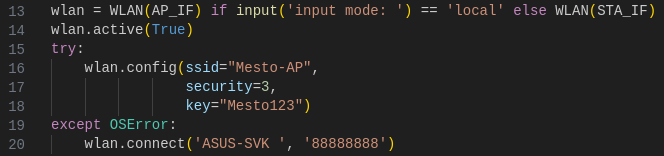
\includegraphics[width=0.8\textwidth]{./graphics/img/image22.png}
	\caption{подключение к сети}
	\label{fig:img22}
\end{figure}

На рисунке \ref{fig:img22} показано подключение к сети. Здесь создаётся экземпляр класса WLAN в раздающем или принимающем варианте соответственно, а затем активируется. Далее использован механизм обработки исключений, который пытается настроить собственную сеть, а при неудаче подключается к существующей сети. Данный код использует особенность создаваемого экземпляра, который может выполнить только одно из указанных действий, а при попытке выполнения другого возвращает исключение.

\begin{figure}[h!]
	\centering
	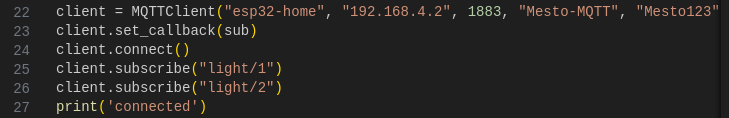
\includegraphics[width=0.9\textwidth]{./graphics/img/image27.png}
	\caption{подключение к mqtt-брокеру}
	\label{fig:img27}
\end{figure}

Здесь показано подключение к mqtt-брокеру. Важно, что уведомление о подключении приходит только после подключения к Mosquitto, ведь до него нет полезного соединения. Также этот код осуществляет подписку на топики.

Данный код просто объявляет переменные для обмена статусом светодиодов, управления светодиодами и датчиками соответственно.

\begin{figure}[h!]
	\centering
	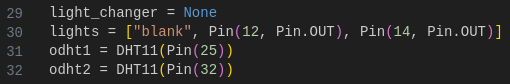
\includegraphics[width=0.8\textwidth]{./graphics/img/image12.png}
	\caption{объявление важных переменных}
	\label{fig:img12}
\end{figure}

\begin{figure}[h!]
	\centering
	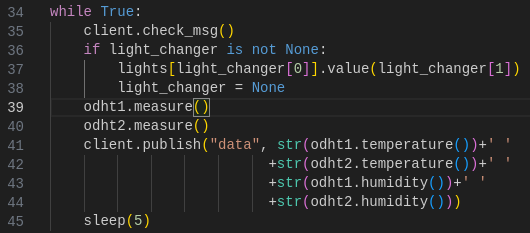
\includegraphics[width=0.8\textwidth]{./graphics/img/image34.png}
	\caption{тело рабочего цикла программы}
	\label{fig:img34}
\end{figure}

Теперь представлено тело рабочего цикла программы. Здесь проверяется наличие новых сообщений во всех топиках, на которые есть подписка, а затем назначается новое значение включённости светодиодам. Далее измеряются температура и влажность, которые собиются в одну строку для удобства передачи и публикуются в топик data. После этого всего идёт ожидание в 5 секунд и цикл повторяется.

\subsection{Особенности реализации}

В данном разделе описывается работа над запуском сервера и микроконтроллера, а также наладкой связи между ними.

Как операционная система для сервера Mosquitto была выбрана Gentoo Linux. Для установки Mosquitto использовался emerge, при этом для снятия маскировки некоторых пакетов пришлось править конфигурационные файлы через терминал в силу особенностей установленной системы с помощью текстового редактора nano и средств управления файловой системой rm \& mkdir.

Также предварительной прошивки и настройки требовал микроконтроллер. Для его прошивки потребовалась программа esptool, которая также есть в репозиториях portage и сам файл прошивки с официального сайта. Инструкция использована с сайта micropython.org. Также для продуктивной разработки под ESP32 используется thonny IDE, которая устанавливается через pip, но при попытке установить в общее пространство системы, но процесс был прерван системой из-за ошибки, заключающейся в том, что общее пространство уже контролируется пакетным менеджером portage. Данное ограничение получилось обойти через создание виртуального окружения с помощью venv.

Следующим шагом стала настройка сети. Было предусмотрено 2 варианта: работа в локальной сети, создаваемой ESP32 и работа в сети с выходом в интернет, создаваемой роутером. Переключение между вариантами соединения производится посредством введения команды local в момент установки соединения либо пропуска поля ввода. Для обоих вариантов было необходимо узнать IP адрес сервера, что было сделано командой ip. Далее адрес был использован в программе микроконтроллера и подключение успешно установлено. Особенности каждого из вариантов подключения со стороны микроконтроллера можно увидеть выше по тексту. Со стороны сервера подключение всегда производится командой nmcli с указанием SSID и пароля сети. Также nmcli имеет функцию хранения паролей, поэтому вводить их требуется только при первом подключении.

При настроенной сети связь с mqtt-брокером уже не вызвала трудностей и данные были успешно переданы с датчиков на сервер.

\chapter{Система компьютерного зрения}

\section{Выбор ИИ для проекта}

Искусственный Интеллект играет важную роль в различных сферах человеческой деятельности, включая область умных домов. В нашем проекте умного дома, ИИ используется для обнаружения силуэтов людей на придомовой территории с целью обеспечения работы охранной системы. 

Одной из основных функций ИИ в нашем проекте является обнаружение силуэтов людей. Для этого применяется система компьютерного зрения, работающая на камерах видеонаблюдения для непрерывного мониторинга придомовой территории. Благодаря ИИ, система способна точно обнаруживать силуэты людей, двигающихся в зоне обзора камер.

Другой важной функцией ИИ в нашем проекте является обеспечение работы охранной системы. Используя данные о силуэтах людей, система определяет наличие посторонних лиц на территории дома. В случае обнаружения проникновения, охранная система автоматически отправляет уведомление владельцу умного дома о возможной угрозе.

Применение Искусственного Интеллекта в системе компьютерного зрения нашего умного дома обеспечивает надежную защиту и моментальное реагирование на потенциальные угрозы безопасности. Благодаря ИИ, владелец умного дома может быть уверен в надежной защите своей территории и оперативном реагировании на любые возможные инциденты.

Таким образом, использование Искусственного Интеллекта в нашем проекте умного дома не только повышает уровень безопасности, но и обеспечивает комфорт и уверенность владельцу, что его территория надежно защищена.

В мире искусственного интеллекта существует несколько типов, включая слабый и сильный ИИ. Слабый ИИ ограничен в своих возможностях и решает задачи в рамках конкретной области, например, системы распознавания речи или обработки изображений. Сильный ИИ, наоборот, обладает способностью обучаться и принимать решения в различных областях, как человек. Кроме того, существуют экспертные системы, которые используют знания экспертов в виде правил для принятия решений, и нейронные сети, которые моделируют работу человеческого мозга.

Для нашего проекта умного дома подходит использование слабого ИИ, а именно системы компьютерного зрения на основе нейронных сетей. Это позволяет нам обнаруживать и классифицировать объекты на видео, такие как люди, транспортные средства и животные, с высокой точностью.

\section{Выбор технологического стека}
Для разработки программного обеспечения нашего проекта мы выбрали язык программирования Python, который получил широкую популярность и имеет богатую экосистему инструментов и библиотек для машинного обучения и обработки данных. Python обеспечивает гибкость и простоту в разработке, что позволяет создавать эффективные и масштабируемые приложения.

Для реализации системы компьютерного зрения мы выбрали библиотеку OpenCV, которая предоставляет множество функций для работы с изображениями и видео. OpenCV обеспечивает высокую производительность и гибкость в обработке видео и изображений. В частности, мы использовали нейросеть YOLOv8, которая является одной из наиболее популярных и эффективных нейросетей для обнаружения объектов на видео. YOLOv8 обеспечивает высокую точность и скорость обнаружения объектов, что позволяет использовать ее в различных приложениях, включая систему компьютерного зрения для нашего проекта умного дома.

\section{Реализация}

В нашем проекте мы использовали встроенную камеру от ноутбука в качестве источника видеопотока для системы компьютерного зрения. Для обработки видеоданных и обнаружения людей мы запустили нейросеть YOLOv8 на том же ноутбуке. Этот выбор позволил нам минимизировать затраты на оборудование и увеличить скорость быстродействия системы.

Мы настроили нейросеть YOLOv8 для обнаружения силуэтов людей на видеопотоке с камеры. Это включало в себя выбор соответствующей модели нейросети, ее обучение на обучающем наборе данных и настройку параметров для достижения оптимальной производительности.

На ноутбуке была запущена охранная программа, которая интегрировала работу камеры, нейросети YOLOv8 и телеграмм бота. Программа непрерывно мониторила видеопоток с камеры, передавала его на обработку нейросети для обнаружения людей и отправляла уведомления через телеграмм бота в случае обнаружения посторонних лиц на территории дома.           

\textbf{Алгоритм работы охранной системы:}

\begin{figure}[h!]
	\centering
	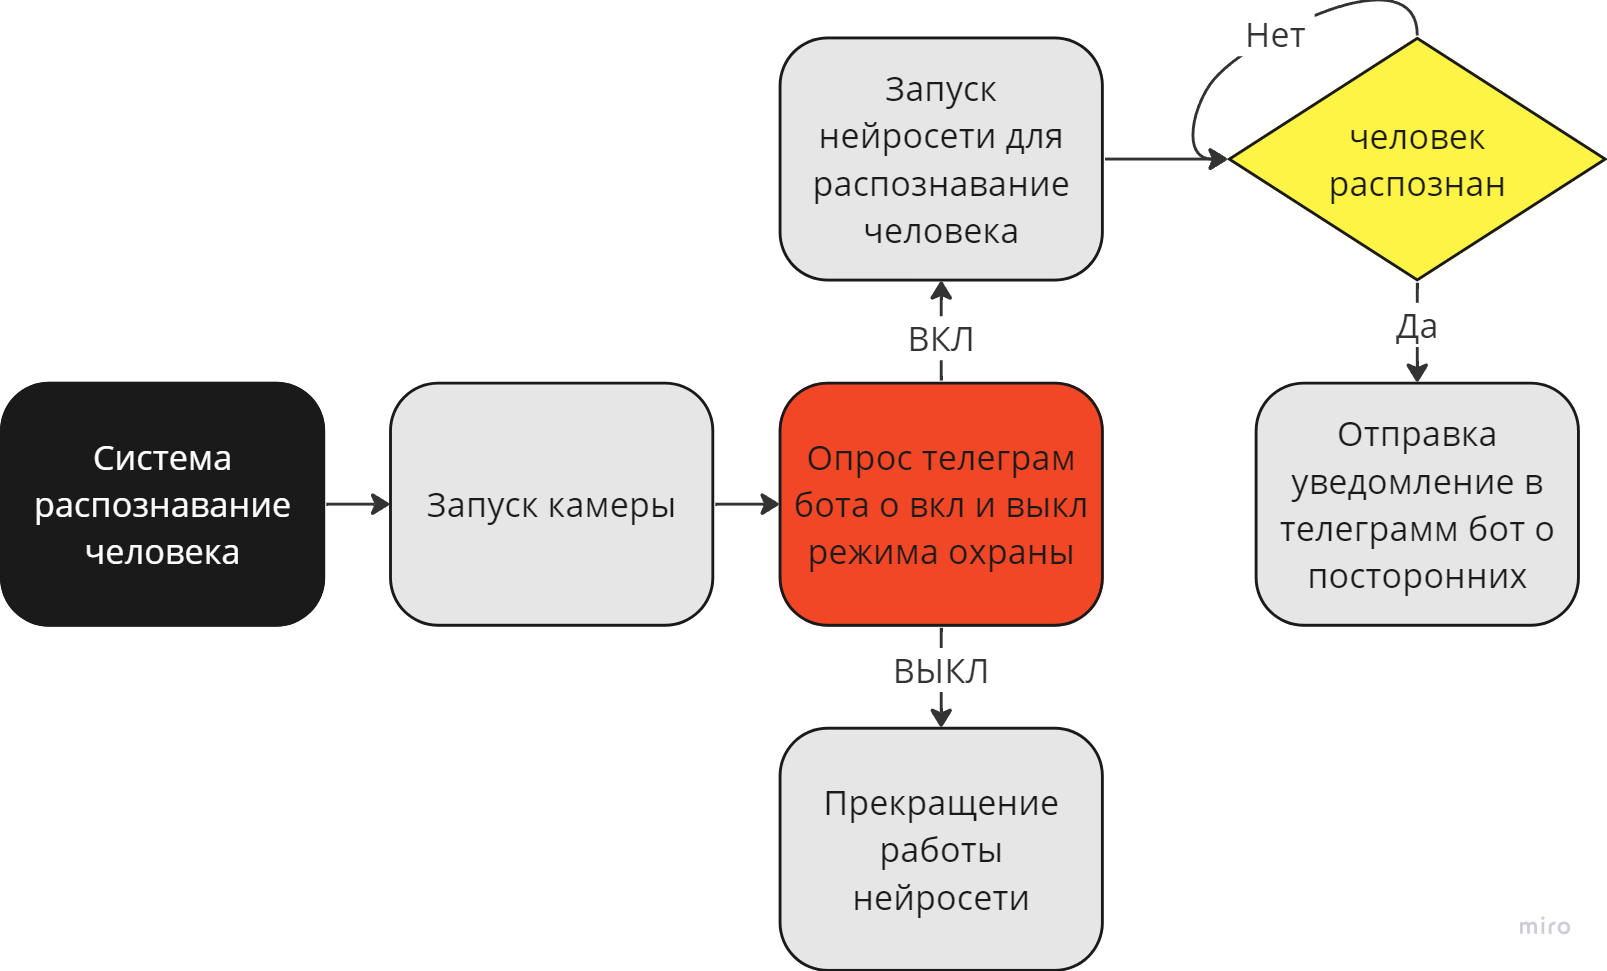
\includegraphics[width=0.8\textwidth]{./graphics/img/image26.png}
	\caption{алгоритм работы охранной системы.}
	\label{fig:img26}
\end{figure}

\subsection{Структура программы:}

Программа охранной системы состоит из двух основных Python файлов:

\textbf{Основной файл обработки видеопотока:}
\\
Этот файл отвечает за обработку видеопотока с камеры и обнаружение нарушений безопасности на придомовой территории. Он включает в себя инициализацию камеры, обработку видеопотока с использованием модели YOLOv8 для обнаружения людей, а также отправку уведомлений через Телеграм бота в случае обнаружения нарушения.

\textbf{Файл с Телеграм ботом:}
\\
Этот файл содержит код Телеграм бота, который обрабатывает команды о включении и выключении охранной системы. Бот принимает команды от пользователя через интерфейс Телеграм мессенджера и управляет работой охранной системы, например, включая или отключая отправку уведомлений о проникновении.

\textbf{Взаимодействие между файлами:}
\\
Для согласованной работы между основным файлом обработки видеопотока и файлом с Телеграм ботом используется текстовый файл "send\_photos.txt". Этот файл служит для передачи информации о необходимости отправки фотографий в Телеграм при обнаружении нарушений безопасности.

Телеграм бот обрабатывает команды пользователя и записывает соответствующие значения в текстовый файл. При получении команды "/photocheck" бот изменяет состояние переменной `send\_ph` и записывает соответствующее значение ("отправлять фото" или "не отправлять фото") в файл "send\_photos.txt".

\begin{figure}[h!]
	\centering
	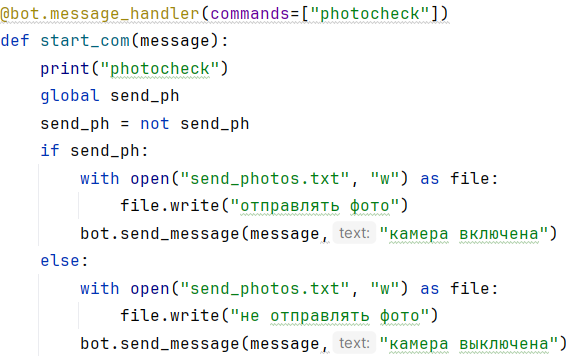
\includegraphics[width=0.8\textwidth]{./graphics/img/image15.png}
	\caption{обработка команды "/photocheck".}
	\label{fig:img15}
\end{figure}

В основном цикле программы осуществляется чтение значения из текстового файла "send\_photos.txt" для определения, нужно ли отправлять фотографии в Телеграм бота при обнаружении нарушений. Если значение в файле указывает на необходимость отправки фотографий и на кадре обнаружены нарушения безопасности, то программа осуществляет отправку фотографии через Телеграм бота.

\begin{figure}[h!]
	\centering
	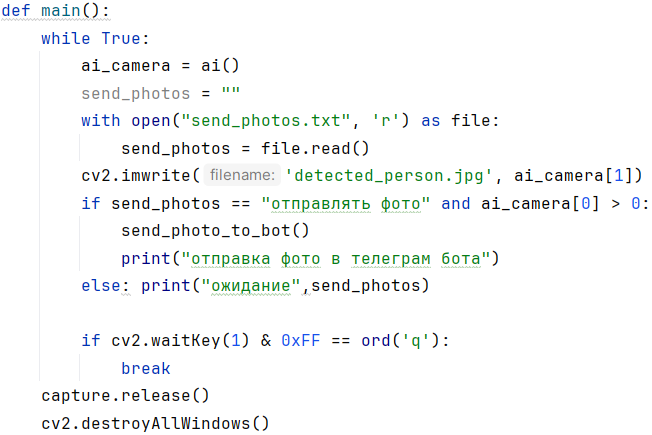
\includegraphics[width=0.8\textwidth]{./graphics/img/image35.png}
	\caption{функция main().}
	\label{fig:img35}
\end{figure}

Главный цикл программы продолжается до момента, когда пользователь не прерывает его. В этом цикле вызывается функция `ai()` для обработки каждого кадра с камеры. В зависимости от настроек, указанных в файле \verb|"send_photos.txt"|, и наличия обнаруженных нарушений, может быть отправлено уведомление с фотографией в Телеграм.

\textbf{Функция отправки фотографии в Телеграм:}

\begin{figure}[h!]
	\centering
	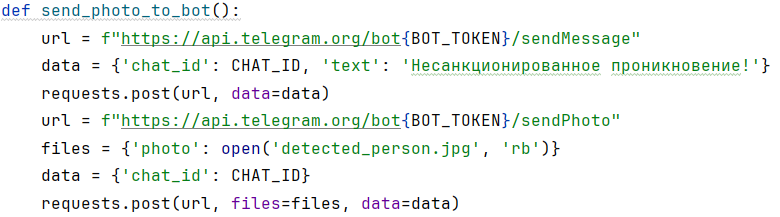
\includegraphics[width=0.8\textwidth]{./graphics/img/image33.png}
	\caption{функция отправки фотографии в Телеграм.}
	\label{fig:img33}
\end{figure}

Создана функция `send\_photo\_to\_bot()`, которая отвечает за отправку уведомления о проникновении через Телеграм бота. При обнаружении нарушения она отправляет уведомление в указанный чат, прикрепляя фотографию с камеры, на которой было обнаружено нарушение.

\textbf{Функция обработки видеопотока с камеры:}

\begin{figure}[h!]
	\centering
	\label{fig:img21}
	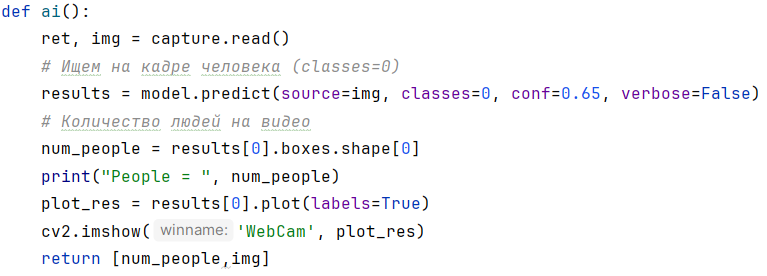
\includegraphics[width=0.8\textwidth]{./graphics/img/image21.png}
	\caption{функция обработки видеопотока с камеры.}
\end{figure}

Разработана функция `ai()`, которая отвечает за обработку видеопотока с камеры. Она использует модель YOLOv8 для обнаружения людей на кадрах с определенным уровнем уверенности и выводит количество обнаруженных людей. При обнаружении нарушения программа отображает на кадре прямоугольники вокруг обнаруженных объектов.

\bfseries
Основной цикл программы:\\*
\hspace*{11.5mm} Главная функция:\\*

\begin{figure}[!h]
	\centering
	\label{fig:img17}
	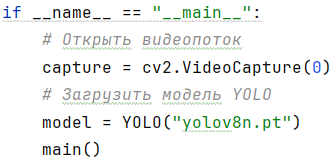
\includegraphics[width=0.5\textwidth]{./graphics/img/image17.png}
	\caption{главная функции.}
\end{figure}

\mdseries
Чтобы обеспечить гибкость и модульность программы, в конце скрипта добавлен блок условия \verb|if __name__ == "__main__":|. Этот блок позволяет запускать код только в случае, если файл выполняется непосредственно, а не импортируется как модуль в другой скрипт.

\chapter{Разработка web-сайта.}

Перед тем, как начать делать сайт, мы решили определить потребности нашей целевой аудитории.

В первую очередь веб-страница должна быть доступной для всех людей. Это включает в себя использование семантического HTML для правильного структурирования контента, а также обеспечение возможности навигации с клавиатуры. 

Помимо этого интерфейс должен быть понятным и лёгким для восприятия, предоставляя пользователю простые инструкции для управления. Также управление сайтом должно быть логичным и последовательным для того, чтобы пользователь легко ориентировался и понимал, что происходит на странице. Кроме того, элементы дизайна и функциональности веб-страницы должны быть согласованы и создавать цельное впечатление, обеспечивая удобство использования.

\section{Анализ существующих web-страниц}

После анализа потребностей нашей целевой аудитории мы решили проанализировать сайты, которые уже существуют.

\begin{enumerate}
	\item Умный дом с Алисой [1]3
	Дизайн и визуальное оформление страницы очень гармонично смотрятся, все расположено понятно для пользователя. Шрифт и композиция соответствуют целевой аудитории. Навигация и удобство использования выделяются на фоне других страниц, так как основные разделы размещены в привычных местах, что делает интерфейс более понятным. Сайт также адаптируется под различные устройства. Особенно привлекательными на сайте являются функциональность и интерактивность, такие как формы обратной связи, возможность комментирования, интерактивные элементы и другие функции. Интерфейс устраивает пользователей.
	
	\item Умный дом Korolab4
	Korolab имеет удобный интерфейс, поскольку все структурировано по этажам. Дизайн и оформление простые и понятные. Шрифт и композиция не выделяются, все размещено стратегически. Однако сайт плохо адаптируется под разные устройства, поскольку в мобильном приложении не выглядит также эстетично, как на веб-странице. Отзывы пользователей положительные относительно интерфейса.
\end{enumerate}
	
\section{Создание дизайна интерфейса}

Так как нашей целевой аудиторией являются молодые семьи с детьми (возраст родителей от 25 до 35 лет), наша веб-страница должна быть простой, удобной в использовании и понятной для пользователей. Также на сайте должны отображаться актуальные данные с датчиков в доме. Помимо этого, для удобства пользователей мы решили внедрить в сайт управление освещением.

\begin{figure}[h!]
	\centering
	\label{fig:img28}
	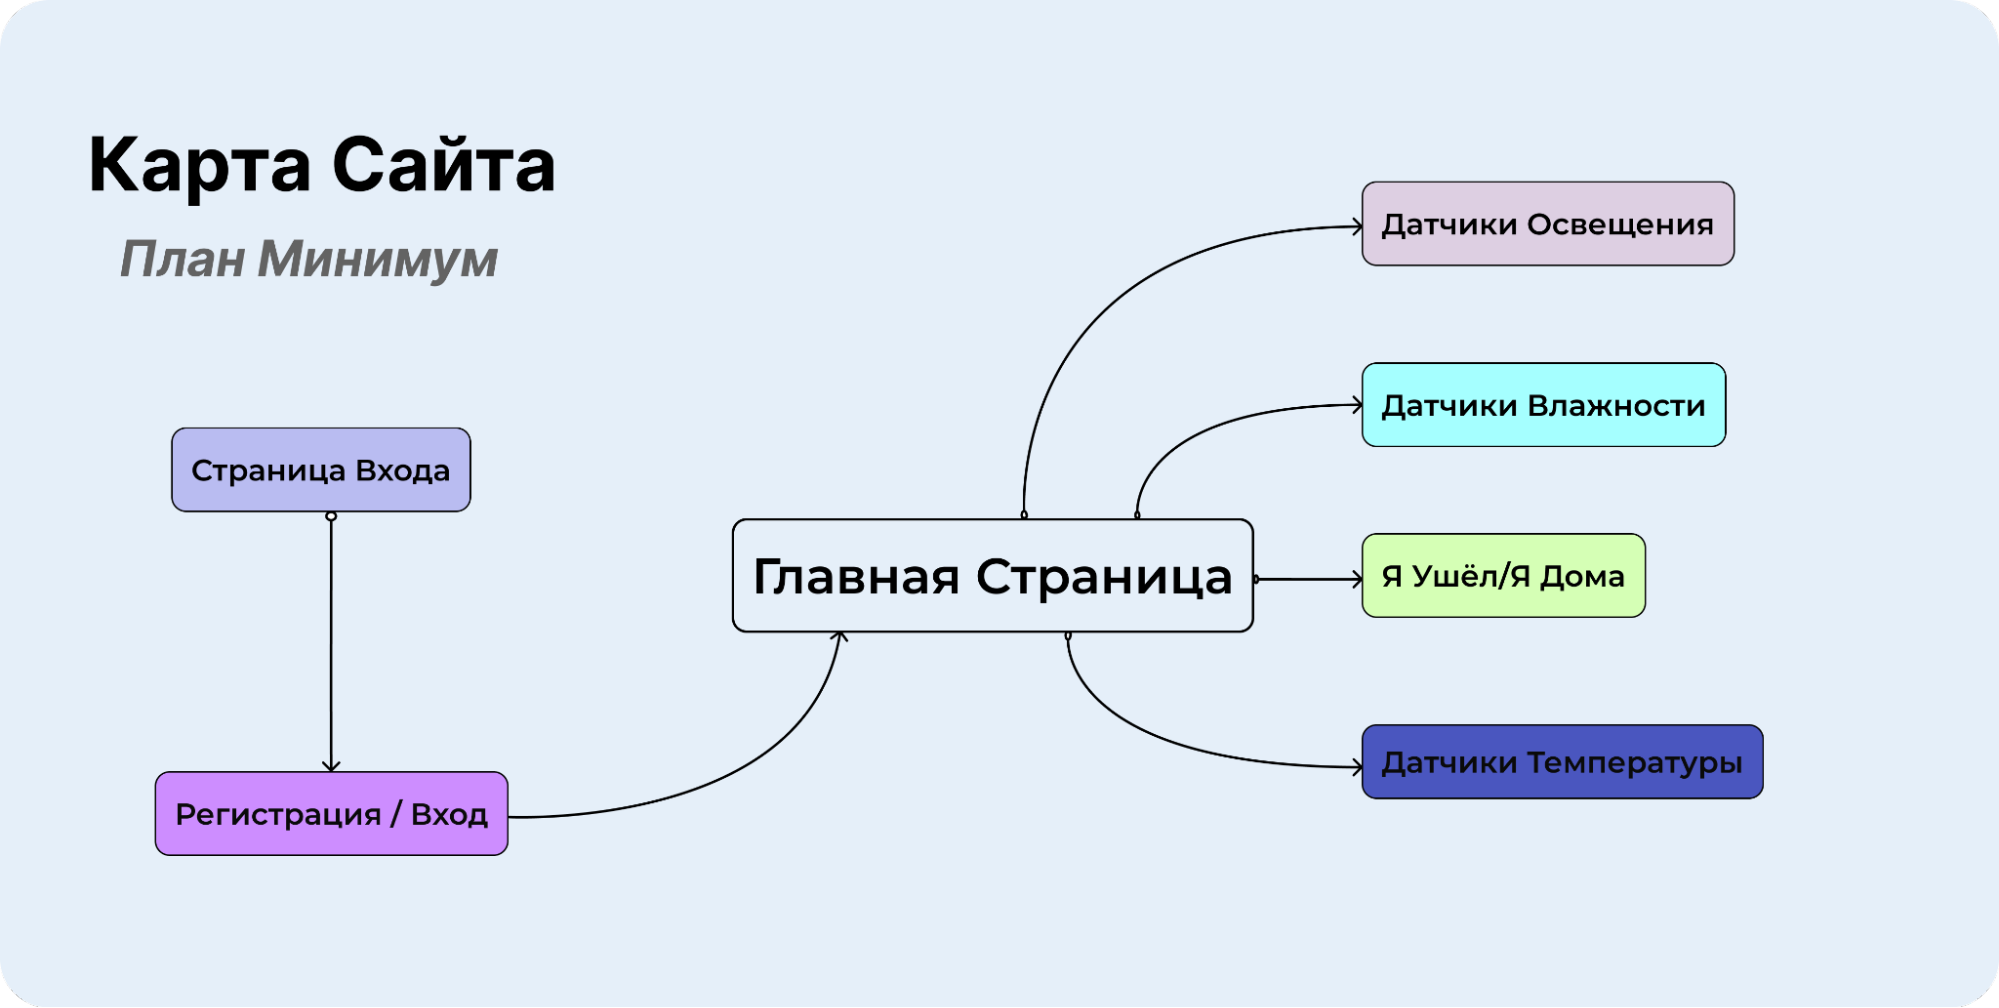
\includegraphics[width=0.8\textwidth]{./graphics/img/image28.png}
	\caption{карта сайта (план “Минимум”).}
\end{figure}

Для понимания того, как будет работать веб-страница мы решили сделать карты сайта. Оценивая наши возможности мы создали план минимум (который мы точно должны сделать), а также план максимум (который было бы хорошо сделать, если это получится).

Изначально мы планировали, чтобы пользователь входил на сайт при помощи пароля, но, после того, как мы решили сделать бота в Telegram, где пользователь будет входить в управление своим домом при помощи своего ID, мы решили пока что это не реализовывать. Также в плане минимум мы решили реализовывать одностраничный сайт, на котором можно просматривать информацию с датчиков, а также регулировать освещённость  на первом и втором этаже. Помимо этого, в начале мы думали, включать и отключать охранную систему прямо на сайте, но в последствии мы поняли, что будет гораздо удобнее это делать в Telegram-боте, нежели на сайте, так как уведомления о несанкционированном проникновении быстрее просматривать в Telegram и фото в телеграм прислать можно быстрее.

\begin{figure}[h!]
	\centering
	\label{fig:img20}
	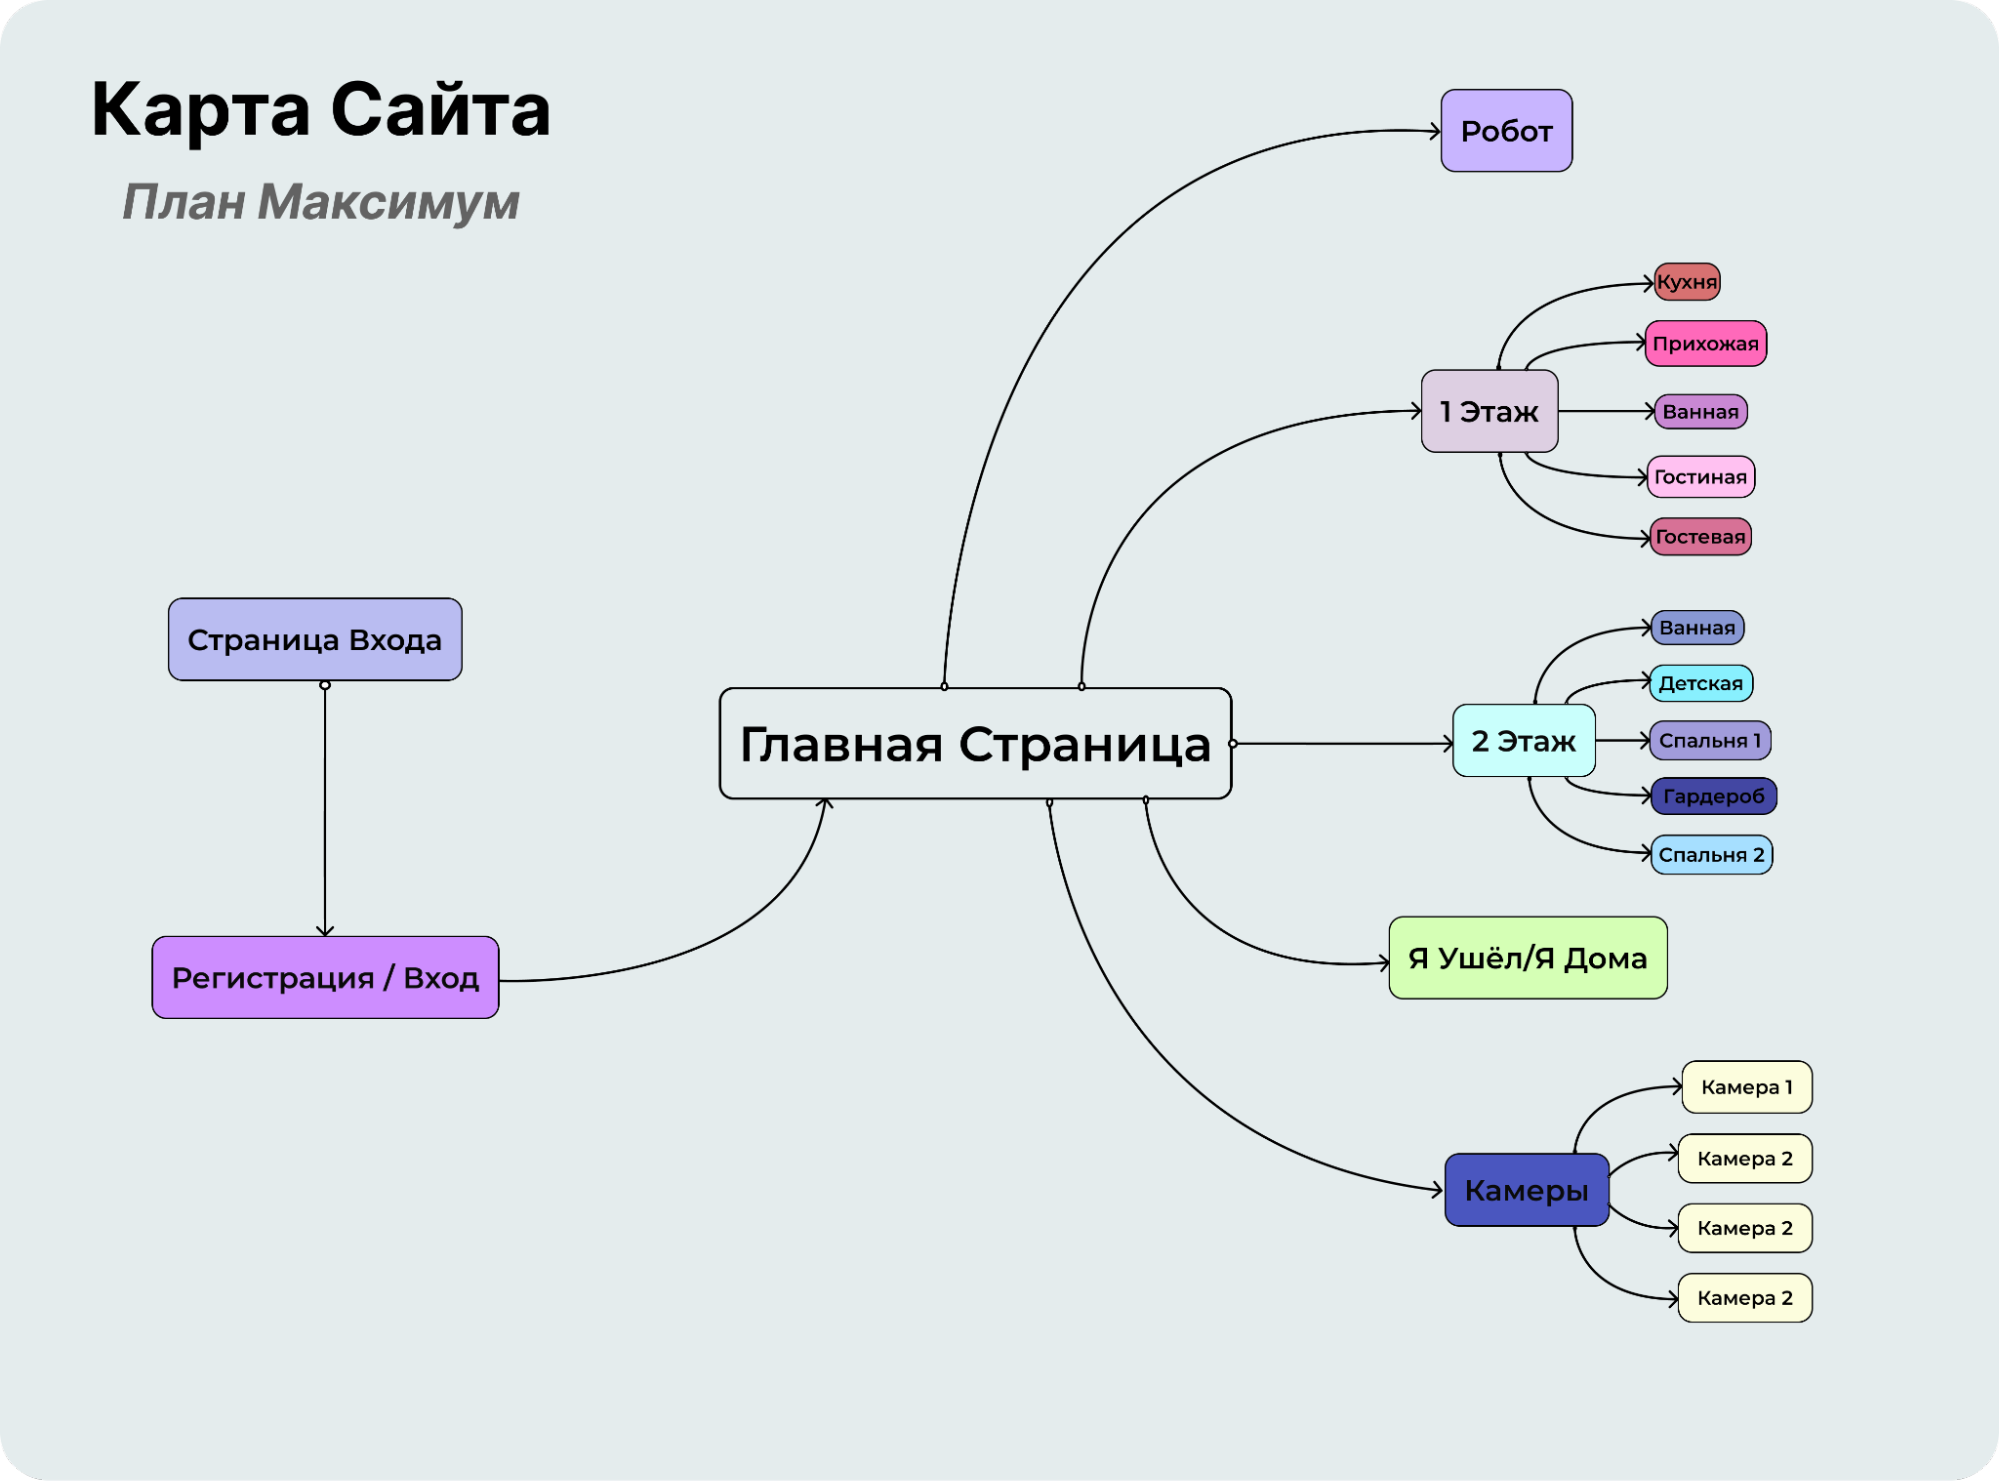
\includegraphics[width=0.8\textwidth]{./graphics/img/image20.png}
	\caption{карта сайта (план “Максимум”).}
\end{figure}

В плане максимум мы планировали сделать многостраничный сайт для того, чтобы просматривать все данные с датчиков и регулировать все параметры в каждой комнате отдельно. Конечно же это гораздо удобнее для пользователя, но в рамках модуля мы не успели это реализовать, поэтому данный план мы решили выполнить в будущем.

После того, как определились со структурой нашего сайта мы перешли к дизайну. Мы стремились сделать его простым, лаконичным и удобным для пользователя. Мы уделили особое внимание  расположению каждого элемента, чтобы при входе на страницу пользователю сразу было понятно, где что находится. Именно благодаря простому дизайну человеку не придётся тратить много времени на поиск того или иного элемента. Большинство объектов размещены именно там, где их ожидают увидеть большинство пользователей, чтобы процесс взаимодействия был интуитивно понятен каждому. Также в футере нашего сайта мы разместили ссылку и QR-код на Telegram-бота для удобства пользователя.

Для создания дизайна мы использовали Figma, так как она  предлагает широкий выбор инструментов для создания дизайна интерфейса. Также в Figma очень удобно работать командой, она позволяет нескольким пользователям работать над проектом одновременно, обмениваться комментариями и видеть изменения в реальном времени. Это делает процесс разработки более эффективным и удобным для командной работы. Также в Figma можно взять информацию об объекте (его размеры и позиционирование, цвет, шрифт, текстовые стили и эффекты), что очень удобно для прописывания стилей в CSS.

\begin{figure}[h!]
	\centering
	\label{fig:img30}
	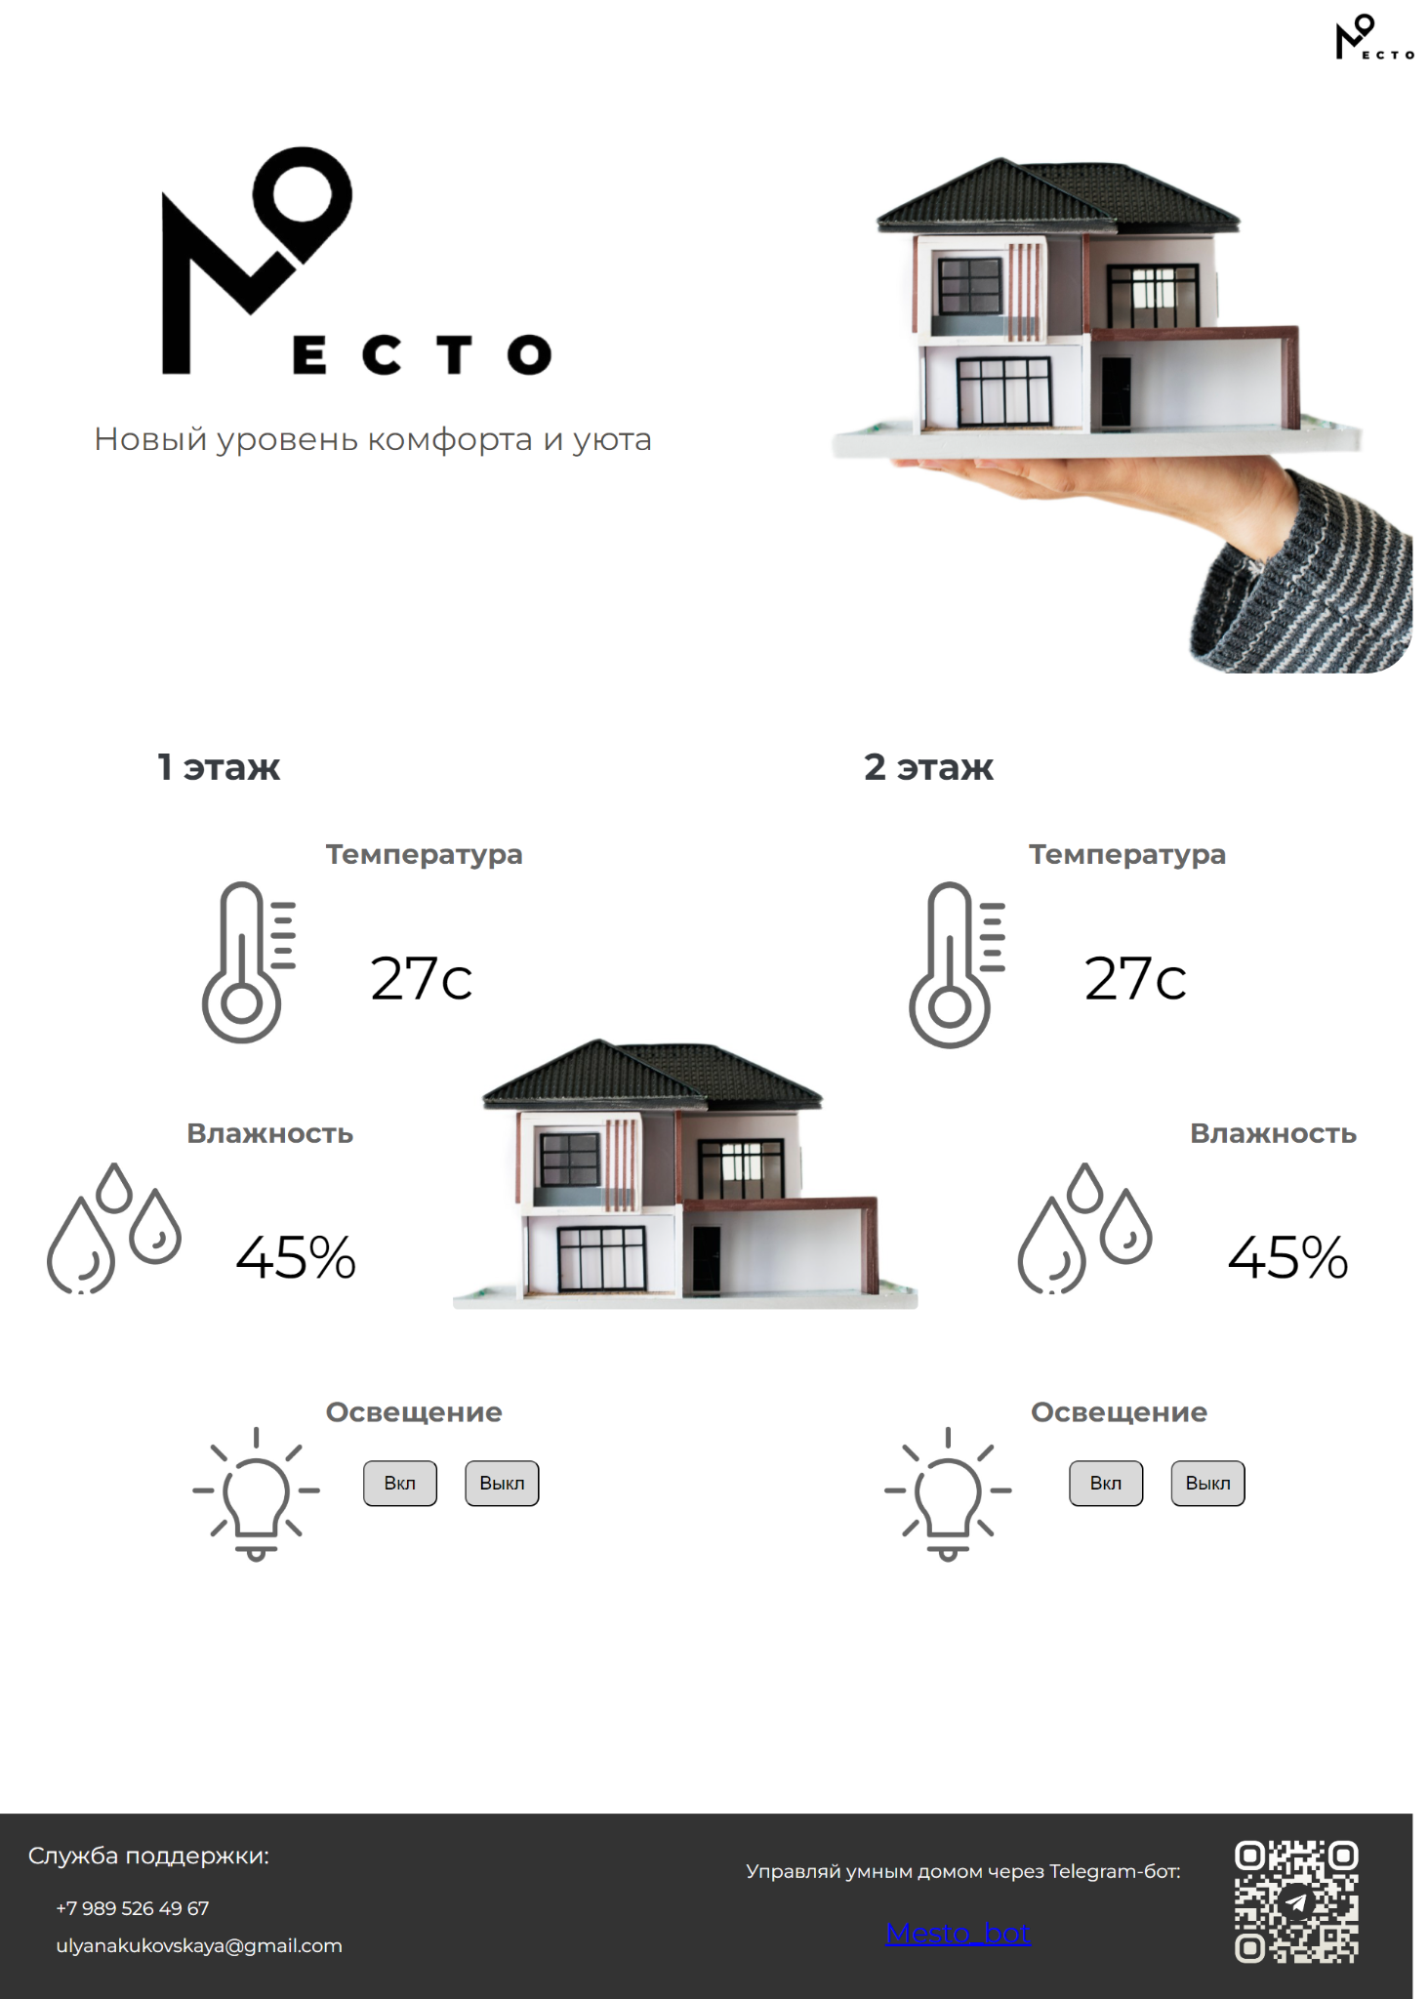
\includegraphics[width=0.8\textwidth]{./graphics/img/image30.png}
	\caption{Дизайн сайта.}
\end{figure}

\section{Разработка веб-страницы}

Мы решили использовать для frontend-разработки редактор кода Sublime text, так как данное приложение является удобным и простым в применении. Для вёрстки сайта мы использовали HTML, а для прописывания стилей элементов - CSS. Мы выбрали именно данные языковые разметки, потому что они являются основополагающими технологиями веб-разработки, также изучение их принципов позволяет понять основы создания веб-страниц. Помимо этого HTML и CSS являются достаточно простыми для изучения и понимания, что делает их отличным выбором для начинающих frontend-разработчиков. 

В HTML документе мы прописывали функции каждого из объектов, а также прописывали типы переменных. Наша страница содержит различные элементы, такие как header и footer, ссылки на стили, изображения, текстовые блоки, а также кнопки.

В заголовке страницы указана метаинформация, такая как кодировка символов, масштаб отображения и ссылки на внешние таблицы стилей:

\begin{figure}[h!]
	\centering
	\label{fig:img39}
	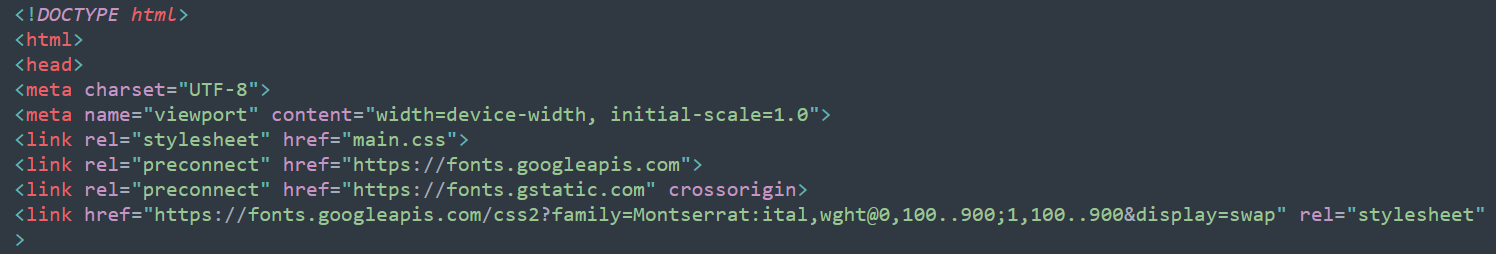
\includegraphics[width=0.8\textwidth]{./graphics/img/image39.png}
	\caption{тег head}
\end{figure}

Также в head указан заголовок веб-страницы, а также иконка, отображаемая во вкладке браузера:

\begin{figure}[h!]
	\centering
	\label{fig:img19}
	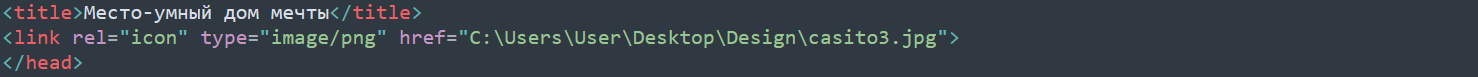
\includegraphics[width=0.8\textwidth]{./graphics/img/image19.png}
	\caption{Заголовок веб-страницы}
\end{figure}

В теле нашей веб-страницы содержатся различные блоки, такие как header:

\begin{figure}[h!]
	\centering
	\label{fig:img38}
	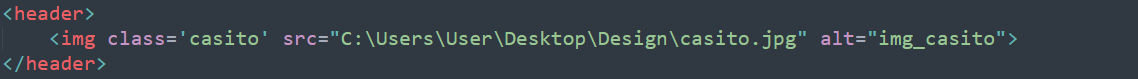
\includegraphics[width=0.8\textwidth]{./graphics/img/image38.png}
	\caption{header сайта}
\end{figure}

Также в body сайта находятся контейнеры с изображениями и текстом, информация о температуре, влажности и освещении, кнопки управления:

\begin{figure}[h!]
	\centering
	\label{fig:img29}
	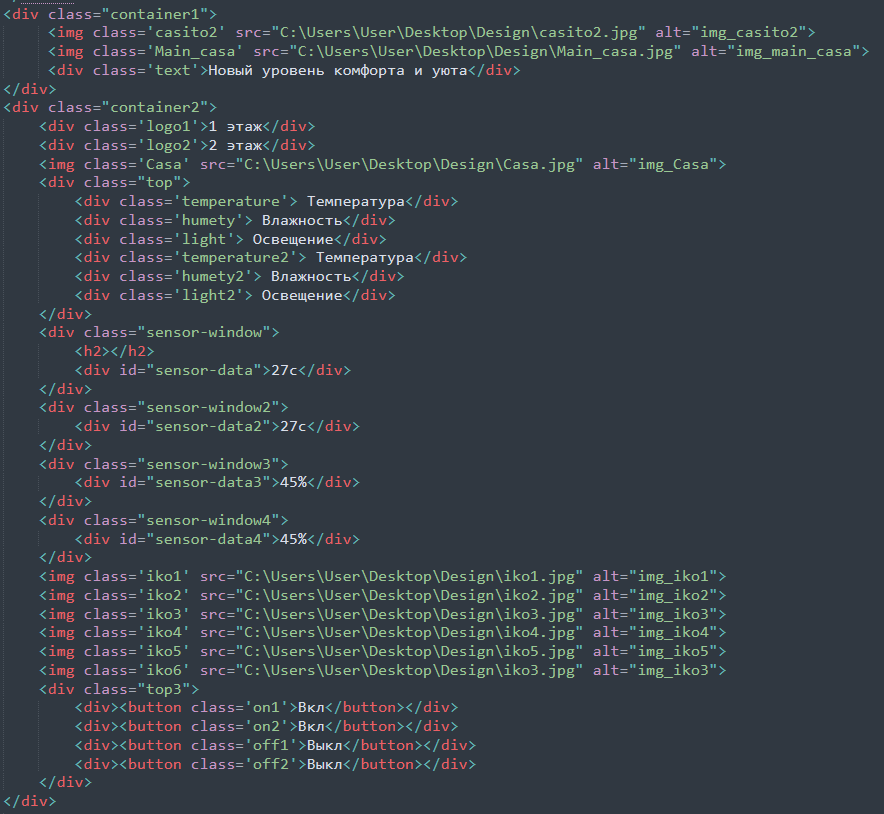
\includegraphics[width=0.8\textwidth]{./graphics/img/image29.png}
	\caption{основная часть сайта}
\end{figure}

В нашем коде мы использовали теги <div class="sensor-window">, которые содержат информацию о датчиках и их показаниях.

В footer мы поместили контактную информацию, QR-код  и ссылку на Telegram-бот для управления умным домом:

\begin{figure}[h!]
	\centering
	\label{fig:img18}
	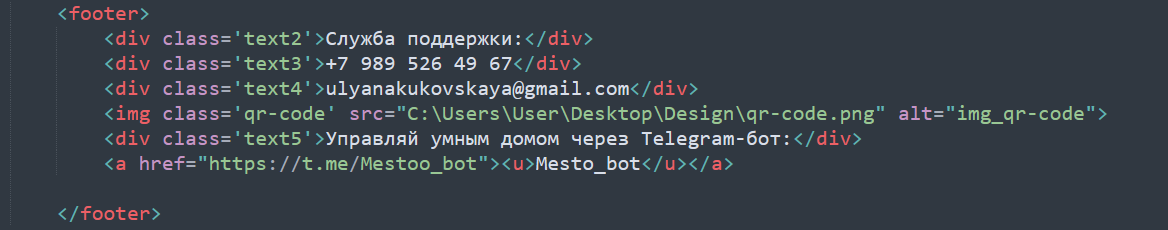
\includegraphics[width=0.8\textwidth]{./graphics/img/image18.png}
	\caption{footer}
\end{figure}

Также в коде присутствуют ссылки на изображения, которые доступны по указанным путям.

В документе CSS мы прописывали стили наших объектов. Мы брали информацию о каждом объекте из Figma, для ускорения процесса. Также для header, body, footer мы прописывали параметры, которые применялись сразу ко всем объектам, находившимся в них:

\begin{figure}[h!]
	\centering
	\label{fig:img16}
	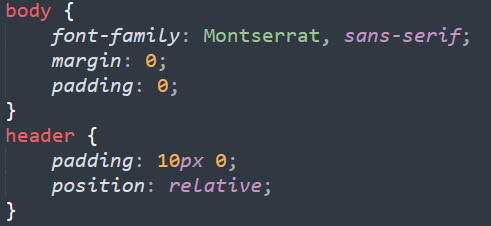
\includegraphics[width=0.8\textwidth]{./graphics/img/image16.png}
	\caption{Стили body, header}
\end{figure}	

\begin{figure}[h!]
	\centering
	\label{fig:img23}
	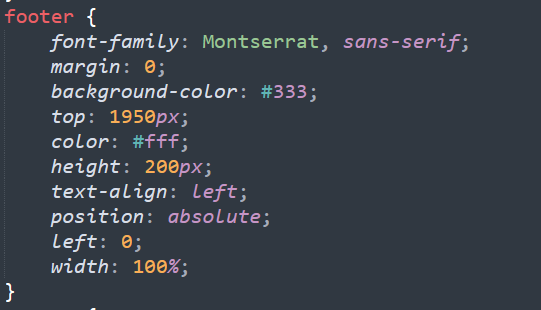
\includegraphics[width=0.8\textwidth]{./graphics/img/image23.png}
	\caption{Стили footer}
\end{figure}	

В процессе разработки мы столкнулись с рядом проблем, так как мы с нуля учились создавать сайт, но несмотря на различные трудности, мы получили большое количество знаний и освоили новые языки программирования.

\chapter{Телеграмм бот}

Бот в Telegram ― это программа, которая автоматизирует определенные задачи и взаимодействие с пользователями в мессенджере Telegram.5

Мы приняли решение воспользоваться телеграмм-ботом в связи с его быстрым и удобным функционалом для отправки и получения информации, как на этапе разработки, так и в процессе эксплуатации.

Плюсы бота которые мы тоже имели в виду при выборе решения. Это то что боты в телеграмме быстро работают и отвечают; ими удобно пользоваться, так как выбор текстовых команд ни у кого не вызывает затруднений; они не нуждаются в установке дополнительного ПО, поскольку любое взаимодействие с ботом осуществляется посредством мессенджера; не затрагивают личные данные без непосредственной команды пользователя и многое другое.

Наш телеграмм бот называется Место по ссылке: https://t.me/Mestoo\_bot 

Цель Место бота: позволяет тебе контактировать с различными функциями умного дома "Место".

\section{Использованные материалы для создания телеграмм бота}

Для понятия какие материалы использовать для создания самого бота с функциями которые мы хотели в него внедрить, они будут более подробно описаны далее: 

Telegram Bot API (https://core.telegram.org/bots/api):

Это официальное API Telegram, предоставляющее возможность создания и взаимодействия с ботами в мессенджере Telegram. API предоставляет различные методы для отправки сообщений, управления подписчиками, работу с медиа-файлами и другие функции. 6

BotFather (https://t.me/botfather):

BotFather является официальным ботом Telegram, который помогает создавать и настраивать новых ботов. Он предоставляет удобный интерфейс для регистрации новых ботов, настройки их параметров, получения токенов доступа и управления командами. 6

Язык программирования Python (https://www.python.org/):

Python - это высокоуровневый язык программирования, который широко используется для разработки телеграм-ботов благодаря своей простоте, мощности и богатой экосистеме библиотек.7

Среда разработки PyCharm (https://www.jetbrains.com/pycharm/):

PyCharm - это интегрированная среда разработки (IDE) для языка программирования Python, предоставляющая широкие возможности для разработки, отладки и управления проектами. 8

Библиотека telebot для работы с Telegram API в Python (https://github.com/eternnoir/pyTelegramBotAPI):

Библиотека telebot - это набор инструментов для работы с Telegram Bot API на языке Python. Она облегчает взаимодействие с API, предоставляя удобные методы для отправки сообщений, обработки команд и работы с медиа-файлами.9

\section{Функции телеграмм бота}

Функции телеграмм ботов, в основном направлены на отправку сообщений, получение информации, обработка команд, уведомление и оповещения, интерактивные элементы как кнопки, работа с базой данных и интеграция с внешними сервисами.

Оценивая нашу целевую аудиторию и цель телеграмм бота, мы внедрили следующие функции для управления умным домом через мессенджер телеграмм:

/Menu (кнопка либо команда)

Если была вызвана команда, то бот будет выводить следующие: 

*Ручные функции*

/temperaturenow - актуальные данные температуры дома

/humiditynow - актуальные данные уровня влаги во воздухе дома

/photocheck - Актуальные фото камер у входов дома

*Автоматические функции*

- Обнаружение посторонних лиц у входа  - отправляется фото этих лиц

- Повышение уровня температуры дома

Если уже будет взаимодействие с кнопкой Menu, она предоставит остальные кнопки для действия

\begin{figure}[h!]
	\centering
	\label{fig:img24}
	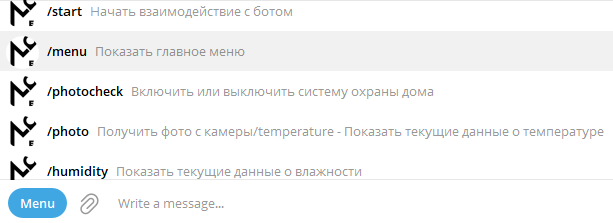
\includegraphics[width=0.8\textwidth]{./graphics/img/image24.png}
	\caption{Изображение меню через функцию кнопки}
\end{figure}

/start (кнопка либо команда)

Для безопасности пользователя бот будет приветствовать его по имени и фамилии, используя данные, предоставленные в Telegram. 

В базе данных бота хранятся идентификационные данные устройства умного дома и его владельца (ID пользователя Telegram, имя и фамилия зашифрованы). При вызове команды /start, если бот не распознает идентификационный номер запросившего, данные дома не будут отображаться при запросе. 

Эта мера безопасности, чтобы предотвратить доступ к конфиденциальным данным дома без соответствующей идентификации пользователя.

/photo (кнопка либо команда)

Это для получения фотографии реального времени с камер находящие в устройстве умного дома.

Также фотографии отправляются автоматически совместно с уведомлением, при обнаружении посторонних лиц.

/photocheck (кнопка либо команда)

Эта функция для включения или выключения камер дома.

/humiditynow (кнопка либо команда)

Она отправляет актуальные данные датчиков устроенных в системе умного дома, данные именно уровня влажности воздуха.

Также, система при обнаружении уровня влажности менее 30\% либо более 80\%, отправляет уведомление о данной информации. Это и за того что слишком высокая влажность воздуха (более 60-70\%) может способствовать развитию плесени, аллергическим реакциям и росту бактерий, что может негативно сказаться на здоровье. 10 А слишком низкая влажность (менее 30\%) может вызывать сухость слизистых оболочек, раздражение глаз, кожи и дыхательных путей. 10

/temperaturenow (кнопка либо команда)

Функция работает наподобие команды и кнопки /humiditynow. Различие заключается в том, что вместо данных уровня влажности воздуха, выводятся данные температуры в реальное время. 

В целом, основная задача телеграм-бота заключается в обеспечении пользователям умного дома удобного способа взаимодействия с виртуальными функциями, позволяя им управлять своим домом через один мессенджер, таким как Telegram. Таким образом, нет необходимости загружать дополнительные приложения для мониторинга и управления.

\chapter{Заключение}

В ходе выполнения данной курсовой работы,  были рассмотрены различные аспекты системы умного дома, начиная с анализа целевой аудитории проекта и заканчивая созданием бота в Telegram.

Анализ целевой аудитории позволил определить основные потребности и предпочтения пользователей, что является ключевым фактором при разработке и внедрении системы умного дома.

Создание системы «Умный дом» включало в себя разработку внешнего вида стенда, взаимодействие элементов системы, алгоритм работы и особенности датчиков. Всё это способствовало созданию функциональной и удобной для использования системы.

Использование системы компьютерного зрения в проекте открывает новые возможности для повышения уровня безопасности и управления различными устройствами в доме

Разработка web-сайта и создание бота в Telegram дополняют функционал системы умного дома, обеспечивая возможность управления и мониторинга через различные платформы.

В целом, данная работа позволила глубже изучить технологии систем умного дома, их применение и перспективы развития. Реализация данных технологий способствует созданию современного и инновационного жилищного пространства, соответствующего потребностям современного общества.

\chapter{Перечень использованных информационных ресурсов}

\begin{enumerate}

    \item \label{i1} Российский рынок умного дома в 2022 году. Продажи, игроки, перспективы – URL: https://mobile-review.com/all/articles/analytics/rossijskij-rynok-umnogo-doma-v-2022-godu-prodazhi-igroki-perspektivy/   

    \item \label{i2} Интернет-Маркетинг для проекта «Умный дом», основываясь на исследованиях яндекса – URL: https://akiwa.ru/blog/internet-marketing-dlya-proekta-umnyy-dom-osnovyvayas-na-issledovaniyakh-yandeksa/

    \item \label{i3} Умный дом Алиса – URL:  https://yandex.ru/alice/smart-home 

    \item \label{i4} Korolab умный дом – URL:https://korolab.ru 

    \item \label{i5} Что такое Telegram и как им пользоваться. GB.RU. – URL: https://gb.ru/blog/chto-takoe-telegram/\#:~:text=%D0%91%D0%BE%D1%82%20%D0%B2%20Telegram%20%E2%80%95%20%D1%8D%D1%82%D0%BE%20%D0%BF%D1%80%D0%BE%D0%B3%D1%80%D0%B0%D0%BC%D0%BC%D0%B0,%2C%20%D0%BA%D0%BE%D1%82%D0%B8%D1%80%D0%BE%D0%B2%D0%BA%D0%B8%2C%20%D1%80%D0%B0%D1%81%D0%BF%D0%B8%D1%81%D0%B0%D0%BD%D0%B8%D0%B5%2C%20%D0%BF%D0%B5%D1%80%D0%B5%D0%B2%D0%BE%D0%B4%D1%8B 

    \item \label{i6} Всё, о чём должен знать разработчик Телеграм-ботов. (2021). Взято с Хабр. – URL: https://habr.com/ru/articles/543676/ 

    \item \label{i7} Amazon Web Services (AWS): "What is Python?" Взято с Amazon Web Services. URL: https://aws.amazon.com/ru/what-is/python/

    \item \label{i8} "Что такое PyCharm?" Взято с Skyeng. – URL: https://skyeng.ru/magazine/chto-takoe-pycharm/ 

    \item "Какую библиотеку на Python выбрать для создания телеграм-бота?" Взято с Хабр. – URL: https://habr.com/ru/companies/otus/articles/771110/ 

    \item \label{i9} "Как влияет влажность воздуха на организм человека": Par-Tuman.ru – URL: https://par-tuman.ru/sferi-primenenia/180-kak-vliyaet-vlazhnost-vozdukha-na-organizm-cheloveka/ 

\end{enumerate}

